\documentclass[]{article}
\usepackage{lmodern}
\usepackage{amssymb,amsmath}
\usepackage{ifxetex,ifluatex}
\usepackage{fixltx2e} % provides \textsubscript
\ifnum 0\ifxetex 1\fi\ifluatex 1\fi=0 % if pdftex
  \usepackage[T1]{fontenc}
  \usepackage[utf8]{inputenc}
\else % if luatex or xelatex
  \ifxetex
    \usepackage{mathspec}
  \else
    \usepackage{fontspec}
  \fi
  \defaultfontfeatures{Ligatures=TeX,Scale=MatchLowercase}
\fi
% use upquote if available, for straight quotes in verbatim environments
\IfFileExists{upquote.sty}{\usepackage{upquote}}{}
% use microtype if available
\IfFileExists{microtype.sty}{%
\usepackage[]{microtype}
\UseMicrotypeSet[protrusion]{basicmath} % disable protrusion for tt fonts
}{}
\PassOptionsToPackage{hyphens}{url} % url is loaded by hyperref
\usepackage[unicode=true]{hyperref}
\hypersetup{
            pdftitle={CSSS/STAT 564 Lab Sessions \#1},
            pdfauthor={Alex Ziyu Jiang},
            pdfborder={0 0 0},
            breaklinks=true}
\urlstyle{same}  % don't use monospace font for urls
\usepackage[margin=1in]{geometry}
\usepackage{color}
\usepackage{fancyvrb}
\newcommand{\VerbBar}{|}
\newcommand{\VERB}{\Verb[commandchars=\\\{\}]}
\DefineVerbatimEnvironment{Highlighting}{Verbatim}{commandchars=\\\{\}}
% Add ',fontsize=\small' for more characters per line
\usepackage{framed}
\definecolor{shadecolor}{RGB}{248,248,248}
\newenvironment{Shaded}{\begin{snugshade}}{\end{snugshade}}
\newcommand{\KeywordTok}[1]{\textcolor[rgb]{0.13,0.29,0.53}{\textbf{#1}}}
\newcommand{\DataTypeTok}[1]{\textcolor[rgb]{0.13,0.29,0.53}{#1}}
\newcommand{\DecValTok}[1]{\textcolor[rgb]{0.00,0.00,0.81}{#1}}
\newcommand{\BaseNTok}[1]{\textcolor[rgb]{0.00,0.00,0.81}{#1}}
\newcommand{\FloatTok}[1]{\textcolor[rgb]{0.00,0.00,0.81}{#1}}
\newcommand{\ConstantTok}[1]{\textcolor[rgb]{0.00,0.00,0.00}{#1}}
\newcommand{\CharTok}[1]{\textcolor[rgb]{0.31,0.60,0.02}{#1}}
\newcommand{\SpecialCharTok}[1]{\textcolor[rgb]{0.00,0.00,0.00}{#1}}
\newcommand{\StringTok}[1]{\textcolor[rgb]{0.31,0.60,0.02}{#1}}
\newcommand{\VerbatimStringTok}[1]{\textcolor[rgb]{0.31,0.60,0.02}{#1}}
\newcommand{\SpecialStringTok}[1]{\textcolor[rgb]{0.31,0.60,0.02}{#1}}
\newcommand{\ImportTok}[1]{#1}
\newcommand{\CommentTok}[1]{\textcolor[rgb]{0.56,0.35,0.01}{\textit{#1}}}
\newcommand{\DocumentationTok}[1]{\textcolor[rgb]{0.56,0.35,0.01}{\textbf{\textit{#1}}}}
\newcommand{\AnnotationTok}[1]{\textcolor[rgb]{0.56,0.35,0.01}{\textbf{\textit{#1}}}}
\newcommand{\CommentVarTok}[1]{\textcolor[rgb]{0.56,0.35,0.01}{\textbf{\textit{#1}}}}
\newcommand{\OtherTok}[1]{\textcolor[rgb]{0.56,0.35,0.01}{#1}}
\newcommand{\FunctionTok}[1]{\textcolor[rgb]{0.00,0.00,0.00}{#1}}
\newcommand{\VariableTok}[1]{\textcolor[rgb]{0.00,0.00,0.00}{#1}}
\newcommand{\ControlFlowTok}[1]{\textcolor[rgb]{0.13,0.29,0.53}{\textbf{#1}}}
\newcommand{\OperatorTok}[1]{\textcolor[rgb]{0.81,0.36,0.00}{\textbf{#1}}}
\newcommand{\BuiltInTok}[1]{#1}
\newcommand{\ExtensionTok}[1]{#1}
\newcommand{\PreprocessorTok}[1]{\textcolor[rgb]{0.56,0.35,0.01}{\textit{#1}}}
\newcommand{\AttributeTok}[1]{\textcolor[rgb]{0.77,0.63,0.00}{#1}}
\newcommand{\RegionMarkerTok}[1]{#1}
\newcommand{\InformationTok}[1]{\textcolor[rgb]{0.56,0.35,0.01}{\textbf{\textit{#1}}}}
\newcommand{\WarningTok}[1]{\textcolor[rgb]{0.56,0.35,0.01}{\textbf{\textit{#1}}}}
\newcommand{\AlertTok}[1]{\textcolor[rgb]{0.94,0.16,0.16}{#1}}
\newcommand{\ErrorTok}[1]{\textcolor[rgb]{0.64,0.00,0.00}{\textbf{#1}}}
\newcommand{\NormalTok}[1]{#1}
\usepackage{longtable,booktabs}
% Fix footnotes in tables (requires footnote package)
\IfFileExists{footnote.sty}{\usepackage{footnote}\makesavenoteenv{long table}}{}
\usepackage{graphicx,grffile}
\makeatletter
\def\maxwidth{\ifdim\Gin@nat@width>\linewidth\linewidth\else\Gin@nat@width\fi}
\def\maxheight{\ifdim\Gin@nat@height>\textheight\textheight\else\Gin@nat@height\fi}
\makeatother
% Scale images if necessary, so that they will not overflow the page
% margins by default, and it is still possible to overwrite the defaults
% using explicit options in \includegraphics[width, height, ...]{}
\setkeys{Gin}{width=\maxwidth,height=\maxheight,keepaspectratio}
\IfFileExists{parskip.sty}{%
\usepackage{parskip}
}{% else
\setlength{\parindent}{0pt}
\setlength{\parskip}{6pt plus 2pt minus 1pt}
}
\setlength{\emergencystretch}{3em}  % prevent overfull lines
\providecommand{\tightlist}{%
  \setlength{\itemsep}{0pt}\setlength{\parskip}{0pt}}
\setcounter{secnumdepth}{0}
% Redefines (sub)paragraphs to behave more like sections
\ifx\paragraph\undefined\else
\let\oldparagraph\paragraph
\renewcommand{\paragraph}[1]{\oldparagraph{#1}\mbox{}}
\fi
\ifx\subparagraph\undefined\else
\let\oldsubparagraph\subparagraph
\renewcommand{\subparagraph}[1]{\oldsubparagraph{#1}\mbox{}}
\fi

% set default figure placement to htbp
\makeatletter
\def\fps@figure{htbp}
\makeatother


\title{CSSS/STAT 564 Lab Sessions \#1}
\author{Alex Ziyu Jiang}
\date{}

\begin{document}
\maketitle

Acknowledgements: the lab session materials are heavily based on our
former course TA, Connor Gilroy's course materials. Check out his
amazing resources here:
\url{https://ccgilroy.github.io/csss564-labs-2019/}

\section{Part 1: Run a simple rstan
example}\label{part-1-run-a-simple-rstan-example}

We first look at how to run a simple demo code in rstan.

\subsection{The eigth schools example}\label{the-eigth-schools-example}

We will be looking at this classic example from Rubin(1981) and Gelman
et. al.(2003).

\begin{itemize}
\tightlist
\item
  Eight schools were tested on the effect on standardized test for
  coaching
\item
  Estimates and standard error of the treatment effect were calculated
\end{itemize}

\begin{longtable}[]{@{}lll@{}}
\toprule
School & Estimated treatment effect & Std. error of treatment
effect\tabularnewline
\midrule
\endhead
A & 28 & 15\tabularnewline
B & 8 & 10\tabularnewline
C & -3 & 16\tabularnewline
D & 7 & 11\tabularnewline
E & -1 & 9\tabularnewline
F & 1 & 11\tabularnewline
G & 18 & 10\tabularnewline
H & 12 & 18\tabularnewline
\bottomrule
\end{longtable}

\subsection{The demo model}\label{the-demo-model}

\begin{align*}
y_j &\stackrel{i.i.d}{\sim} N(\theta_j, \sigma_j^2), j = 1,...,J=8~~\text{(likelihood model)}  \\
\theta_j &\stackrel{i.i.d}{\sim} N(\mu , \tau^2), j = 1,...,J=8~~\text{(prior)} \\
p(\sigma_j,\mu, \tau) &\propto 1 ~~\text{(flat priors)}
\end{align*}

\subsection{breaking down the model}\label{breaking-down-the-model}

\textbf{observables}

\begin{itemize}
\tightlist
\item
  \(y_j\): estimated treatment effects
\item
  \(\sigma_j\): standard error of effect estimated
\item
  \(J\): number of schools
\end{itemize}

\textbf{unknown parameters}

\begin{itemize}
\tightlist
\item
  \(\theta_j\): school treatment effects
\item
  \(\mu\): population treatment effect
\item
  \(\tau\): standard deviation in school treatment effects
\end{itemize}

\subsection{key parts in a stan code}\label{key-parts-in-a-stan-code}

\textbf{required parts}

\begin{itemize}
\tightlist
\item
  data: data to be fed in the stan model
\item
  parameters: unknown parameters in the model; goal of inference
\item
  model: usually includes likelihood and prior
\end{itemize}

\textbf{optional parts}

\begin{itemize}
\tightlist
\item
  transformed parameters: preprocessing the parameter
\item
  generated quantities: preprocessing the results
\end{itemize}

\subsection{\texorpdfstring{the stan code (saved as
`8schools.stan')}{the stan code (saved as 8schools.stan)}}\label{the-stan-code-saved-as-8schools.stan}

(Note: to run this code chunk, save it as a separate file with the
extension name `.stan' under the same directory as this .rmd file.)

\begin{verbatim}
// not run
data {
  int<lower=0> J;         // number of schools 
  real y[J];              // estimated treatment effects
  real<lower=0> sigma[J]; // standard error of effect estimates 

parameters {
  real mu;                // population treatment effect
  real<lower=0> tau;      // standard deviation in treatment effects
}
model {
  theta ~ normal(mu, tau); // prior
  y ~ normal(theta, sigma); // likelihood
}
\end{verbatim}

\textbf{important notes}

\begin{itemize}
\tightlist
\item
  vectorize your data: use y{[}J{]} to specify a vector of length J
\item
  specify the range of your data: standard deviation/error has lower
  bound 0, use lower=0
\item
  the second parameter in normal() is the standard deviation, not the
  variance
\end{itemize}

\subsection{run the model in rstudio}\label{run-the-model-in-rstudio}

After coding the .stan file and saving it to the same directory of our R
script, we can compile it in RStudio.

\begin{Shaded}
\begin{Highlighting}[]
\CommentTok{# feed in the data (match the data part in your stan code)}
\NormalTok{schools_dat <-}\StringTok{ }\KeywordTok{list}\NormalTok{(}\DataTypeTok{J =} \DecValTok{8}\NormalTok{, }
                    \DataTypeTok{y =} \KeywordTok{c}\NormalTok{(}\DecValTok{28}\NormalTok{, }\DecValTok{8}\NormalTok{, }\OperatorTok{-}\DecValTok{3}\NormalTok{,  }\DecValTok{7}\NormalTok{, }\OperatorTok{-}\DecValTok{1}\NormalTok{,}\DecValTok{1}\NormalTok{, }\DecValTok{18}\NormalTok{, }\DecValTok{12}\NormalTok{),}
                    \DataTypeTok{sigma =} \KeywordTok{c}\NormalTok{(}\DecValTok{15}\NormalTok{, }\DecValTok{10}\NormalTok{, }\DecValTok{16}\NormalTok{, }\DecValTok{11}\NormalTok{, }\DecValTok{9}\NormalTok{, }\DecValTok{11}\NormalTok{, }\DecValTok{10}\NormalTok{, }\DecValTok{18}\NormalTok{))}
\CommentTok{# run the stan code }
\NormalTok{fit <-}\StringTok{ }\KeywordTok{stan}\NormalTok{(}\DataTypeTok{file =} \StringTok{"C:}\CharTok{\textbackslash{}\textbackslash{}}\StringTok{Users}\CharTok{\textbackslash{}\textbackslash{}}\StringTok{00000}\CharTok{\textbackslash{}\textbackslash{}}\StringTok{Documents}\CharTok{\textbackslash{}\textbackslash{}}\StringTok{GitHub}\CharTok{\textbackslash{}\textbackslash{}}\StringTok{CSSS-STAT-564}\CharTok{\textbackslash{}\textbackslash{}}\StringTok{lab1}\CharTok{\textbackslash{}\textbackslash{}}\StringTok{8schools.stan"}\NormalTok{, }\DataTypeTok{data =}\NormalTok{ schools_dat,}\DataTypeTok{refresh =} \DecValTok{0}\NormalTok{)}
\end{Highlighting}
\end{Shaded}

We can call stan\_plot to visualize the model output:

\begin{Shaded}
\begin{Highlighting}[]
\KeywordTok{stan_plot}\NormalTok{(fit, }\DataTypeTok{show_density =} \OtherTok{TRUE}\NormalTok{)}
\end{Highlighting}
\end{Shaded}

\begin{verbatim}
## ci_level: 0.8 (80% intervals)
\end{verbatim}

\begin{verbatim}
## outer_level: 0.95 (95% intervals)
\end{verbatim}

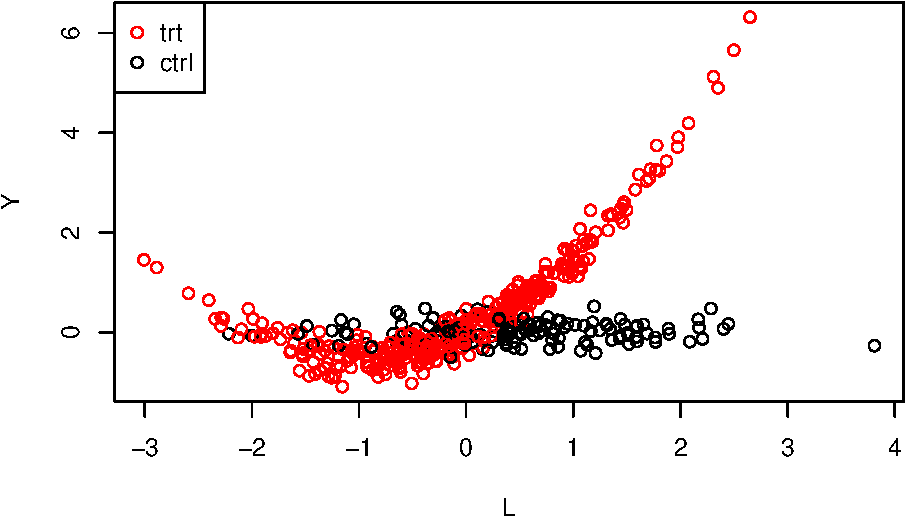
\includegraphics{lab1_files/figure-latex/unnamed-chunk-4-1.pdf}

\section{Part 2: Simulation}\label{part-2-simulation}

\subsection{Simulating by sampling}\label{simulating-by-sampling}

Why is simulation important?

\begin{itemize}
\item
  If you have a known distribution (a prior, or a likelihood) you can
  simulate data from it to understand how it will behave.
\item
  If you don't know a (posterior) distribution, you can still
  approximate it by sampling from it.
\item
  To check the behavior of your model, you can simulate more data from
  the (posterior predictive) distribution using sampled parameter
  values.
\end{itemize}

\subsection{Discrete distribution:
Poisson}\label{discrete-distribution-poisson}

The Poisson distribution is useful for modeling count data; it's a
discrete distribution that only takes on integer values that are
nonnegative. We recall that a Poisson distribution with mean parameter
\(\lambda\) has the following probability mass function:

\begin{align*}
\operatorname{Pr}(X=k)=\frac{\lambda^{k} e^{-\lambda}}{k !}
\end{align*}

To calculate this in RStudio, we can use dpois to analytically calculate
the density for a Poisson distribution with \(\lambda\)=5. (We stop at
an arbitrary large value of \(x\).)

\begin{Shaded}
\begin{Highlighting}[]
\NormalTok{xs <-}\StringTok{ }\DecValTok{0}\OperatorTok{:}\DecValTok{15} \CommentTok{# stop at x=15}
\NormalTok{densities <-}\StringTok{ }\KeywordTok{dpois}\NormalTok{(}\DataTypeTok{x =}\NormalTok{ xs, }\DataTypeTok{lambda =} \DecValTok{5}\NormalTok{) }\CommentTok{# calculates the poisson likelihood for x from 0 to 15 with mean parameter 5}
\NormalTok{df <-}\StringTok{ }\KeywordTok{tibble}\NormalTok{(}\DataTypeTok{x =}\NormalTok{ xs, }\DataTypeTok{densities =}\NormalTok{ densities) }\CommentTok{# create a dataframe with the xs and the densities}
\KeywordTok{ggplot}\NormalTok{(df, }\KeywordTok{aes}\NormalTok{(}\DataTypeTok{x =}\NormalTok{ x, }\DataTypeTok{y =}\NormalTok{ densities)) }\OperatorTok{+}\StringTok{ }\KeywordTok{geom_col}\NormalTok{() }\CommentTok{# plot the densities as columns}
\end{Highlighting}
\end{Shaded}

\begin{center}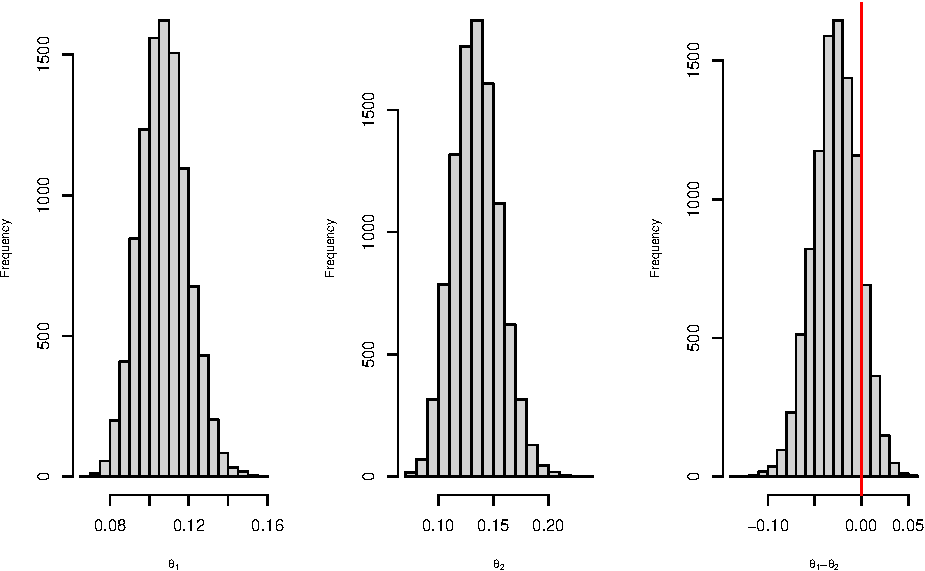
\includegraphics{lab1_files/figure-latex/unnamed-chunk-6-1} \end{center}

Then, if we draw samples from the same distribution, we should get
something close to the theoretical densities (i.e.~the shape of the
histogram of counts should be similar to the shape of the density
function).

To do this, we use the function rpois to generate i.i.d samples from the
Poisson distribution \(\text{Poisson}(\lambda = 5)\).

\begin{Shaded}
\begin{Highlighting}[]
\NormalTok{poisson_samples <-}\StringTok{ }\KeywordTok{rpois}\NormalTok{(}\DataTypeTok{n =}\NormalTok{ nsims, }\DataTypeTok{lambda =} \DecValTok{5}\NormalTok{)}

\CommentTok{# first, plot counts}
\KeywordTok{tibble}\NormalTok{(}\DataTypeTok{samples =}\NormalTok{ poisson_samples) }\OperatorTok
\StringTok{  }\KeywordTok{ggplot}\NormalTok{(}\KeywordTok{aes}\NormalTok{(}\DataTypeTok{x =}\NormalTok{ samples)) }\OperatorTok{+}\StringTok{ }
\StringTok{  }\KeywordTok{geom_bar}\NormalTok{()}
\end{Highlighting}
\end{Shaded}

\begin{center}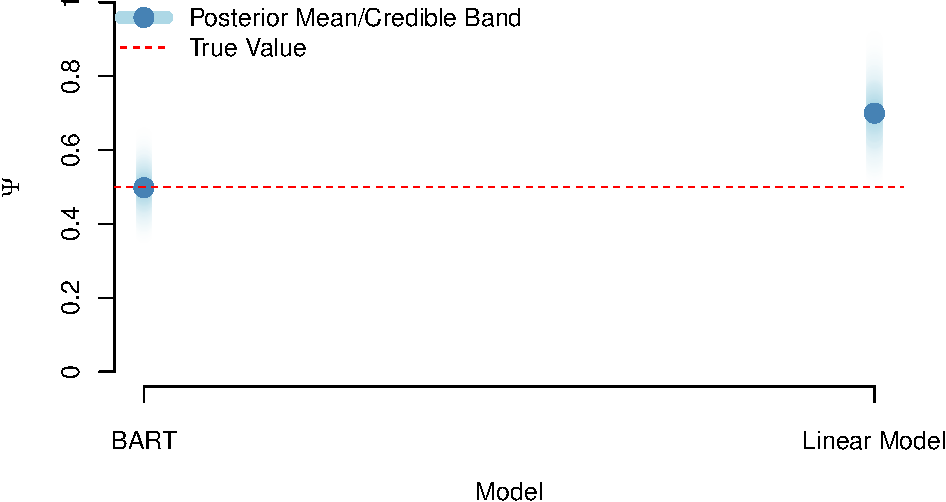
\includegraphics{lab1_files/figure-latex/unnamed-chunk-7-1} \end{center}

We can also overlay these two together:

\begin{Shaded}
\begin{Highlighting}[]
\CommentTok{# plot the density function/mass function of the Poisson density against the bar plot of empirical rates based on samples from the distribution}

\CommentTok{# tally the samples by their values and calculate the rate for each value}
\NormalTok{df2 <-}\StringTok{ }\KeywordTok{tibble}\NormalTok{(}\DataTypeTok{samples =}\NormalTok{ poisson_samples) }\OperatorTok
\StringTok{  }\KeywordTok{count}\NormalTok{(samples) }\OperatorTok
\StringTok{  }\KeywordTok{mutate}\NormalTok{(}\DataTypeTok{frac =}\NormalTok{ n}\OperatorTok{/}\NormalTok{nsims)}

\CommentTok{# overlay the two graphs }
\NormalTok{df }\OperatorTok\StringTok{ }\KeywordTok{ggplot}\NormalTok{(}\KeywordTok{aes}\NormalTok{(}\DataTypeTok{x =}\NormalTok{ x, }\DataTypeTok{y =}\NormalTok{ densities)) }\OperatorTok{+}
\StringTok{  }\KeywordTok{geom_point}\NormalTok{(}\DataTypeTok{size =}\NormalTok{ .}\DecValTok{5}\NormalTok{) }\OperatorTok{+}\StringTok{ }
\StringTok{  }\KeywordTok{geom_line}\NormalTok{() }\OperatorTok{+}\StringTok{  }
\StringTok{  }\KeywordTok{geom_col}\NormalTok{(}\DataTypeTok{data =}\NormalTok{ df2, }\KeywordTok{aes}\NormalTok{(}\DataTypeTok{x =}\NormalTok{ samples, }\DataTypeTok{y =}\NormalTok{ frac))}
\end{Highlighting}
\end{Shaded}

\begin{center}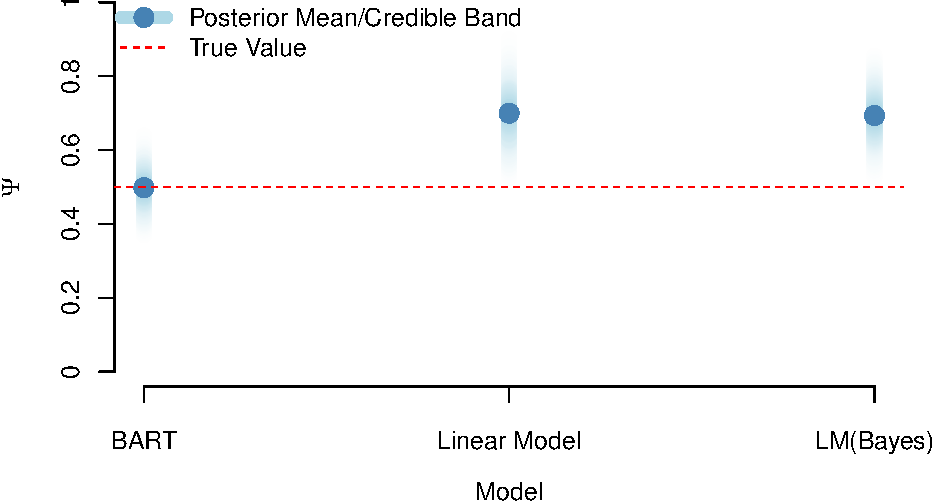
\includegraphics{lab1_files/figure-latex/unnamed-chunk-8-1} \end{center}

\subsection{Continuous distribution:
Gamma}\label{continuous-distribution-gamma}

The gamma distribution is a continuous probability distribution. We can
plot an approximation of the shape from the true densities using a grid
of values. A gamma distribution with shape parameter \(\alpha\) and rate
parameter \(\beta\) has the following probability density function
(beware of the specification of the parameters! If we use the scale
parameter instead of the rate parameter, it is the inverse of
\(\beta\)):

\begin{align*}
f(x)=\frac{\beta^{\alpha}}{\Gamma(\alpha)} x^{\alpha-1} e^{-\beta x}
\end{align*}

We'll use \(\text{Gamma}(2,0.1)\) ---a shape parameter of 2, and a rate
(or inverse scale) parameter of 0.1. Try changing these values and see
how the distribution changes.

\begin{Shaded}
\begin{Highlighting}[]
\CommentTok{# analytic densities: construct a set of grid values from 0 to 120}
\NormalTok{xs <-}\StringTok{ }\KeywordTok{seq}\NormalTok{(}\DecValTok{0}\NormalTok{, }\DecValTok{120}\NormalTok{, }\DataTypeTok{by =} \DecValTok{2}\NormalTok{)}

\CommentTok{# be careful of the parameter: rate or scale?}
\NormalTok{gamma_densities <-}\StringTok{ }\KeywordTok{dgamma}\NormalTok{(}\DataTypeTok{x =}\NormalTok{ xs, }\DataTypeTok{shape =} \DecValTok{2}\NormalTok{, }\DataTypeTok{rate =} \FloatTok{0.1}\NormalTok{)}

\CommentTok{# plot the density values on a line}
\NormalTok{p1 <-}\StringTok{ }\KeywordTok{tibble}\NormalTok{(}\DataTypeTok{x =}\NormalTok{ xs, }\DataTypeTok{densities =}\NormalTok{ gamma_densities) }\OperatorTok
\StringTok{  }\KeywordTok{ggplot}\NormalTok{(}\KeywordTok{aes}\NormalTok{(}\DataTypeTok{x =}\NormalTok{ x, }\DataTypeTok{y =}\NormalTok{ densities)) }\OperatorTok{+}
\StringTok{  }\KeywordTok{geom_point}\NormalTok{(}\DataTypeTok{size =}\NormalTok{ .}\DecValTok{5}\NormalTok{) }\OperatorTok{+}\StringTok{ }
\StringTok{  }\KeywordTok{geom_line}\NormalTok{()}
\NormalTok{p1 }
\end{Highlighting}
\end{Shaded}

\begin{center}\includegraphics{lab1_files/figure-latex/unnamed-chunk-9-1} \end{center}

Since this is a continuous distribution, we'll use a kernel density
(rather than a histogram) to plot the samples.

\begin{Shaded}
\begin{Highlighting}[]
\CommentTok{# densities from samples}
\NormalTok{gamma_samples <-}\StringTok{ }\KeywordTok{rgamma}\NormalTok{(}\DataTypeTok{n =}\NormalTok{ nsims, }\DataTypeTok{shape =} \DecValTok{2}\NormalTok{, }\DataTypeTok{rate =} \FloatTok{0.1}\NormalTok{)}
\NormalTok{df.}\DecValTok{2}\NormalTok{ <-}\StringTok{ }\KeywordTok{tibble}\NormalTok{(}\DataTypeTok{samples =}\NormalTok{ gamma_samples)}
\NormalTok{p2 <-}\StringTok{ }\KeywordTok{data_frame}\NormalTok{(}\DataTypeTok{samples =}\NormalTok{ gamma_samples) }\OperatorTok
\StringTok{  }\KeywordTok{ggplot}\NormalTok{(}\KeywordTok{aes}\NormalTok{(}\DataTypeTok{x =}\NormalTok{ samples)) }\OperatorTok{+}\StringTok{ }
\StringTok{  }\KeywordTok{geom_density}\NormalTok{()}
\end{Highlighting}
\end{Shaded}

\begin{verbatim}
## Warning: `data_frame()` was deprecated in tibble 1.1.0.
## Please use `tibble()` instead.
\end{verbatim}

\begin{Shaded}
\begin{Highlighting}[]
\NormalTok{p2}
\end{Highlighting}
\end{Shaded}

\begin{center}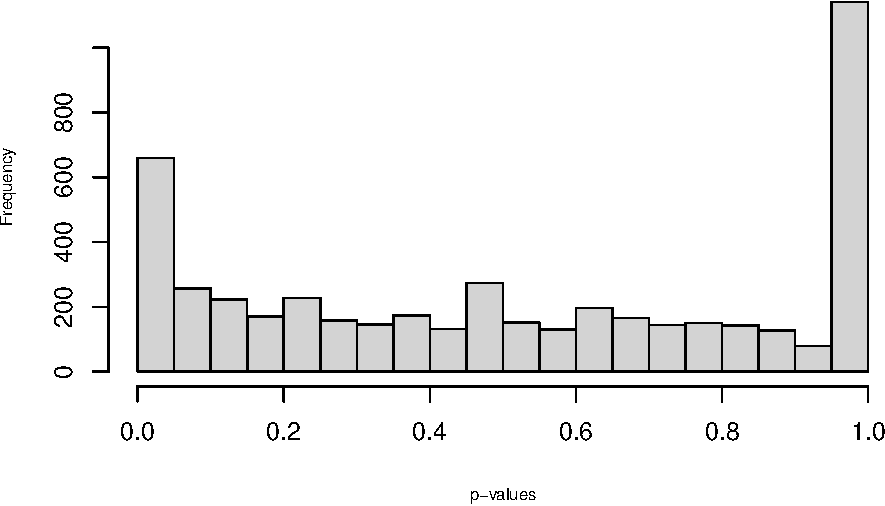
\includegraphics{lab1_files/figure-latex/unnamed-chunk-10-1} \end{center}

If you know the theoretical distribution, another way to compare the
samples to it is with a quantile-quantile plot:

\begin{Shaded}
\begin{Highlighting}[]
\KeywordTok{tibble}\NormalTok{(}\DataTypeTok{samples =}\NormalTok{ gamma_samples) }\OperatorTok
\StringTok{  }\KeywordTok{ggplot}\NormalTok{(}\KeywordTok{aes}\NormalTok{(}\DataTypeTok{sample =}\NormalTok{ samples)) }\OperatorTok{+}\StringTok{ }
\StringTok{  }\KeywordTok{geom_qq}\NormalTok{(}\DataTypeTok{distribution =}\NormalTok{ qgamma, }
          \DataTypeTok{dparams =} \KeywordTok{list}\NormalTok{(}\DataTypeTok{shape =} \DecValTok{2}\NormalTok{, }\DataTypeTok{rate =} \FloatTok{0.1}\NormalTok{)) }\OperatorTok{+}\StringTok{  }\CommentTok{# generate points with coordinates as theoretical and empirical quantiles}
\StringTok{  }\KeywordTok{geom_qq_line}\NormalTok{(}\DataTypeTok{distribution =}\NormalTok{ qgamma,}
               \DataTypeTok{dparams =} \KeywordTok{list}\NormalTok{(}\DataTypeTok{shape =} \DecValTok{2}\NormalTok{, }\DataTypeTok{rate =} \FloatTok{0.1}\NormalTok{)) }\CommentTok{# generate the reference line }
\end{Highlighting}
\end{Shaded}

\begin{center}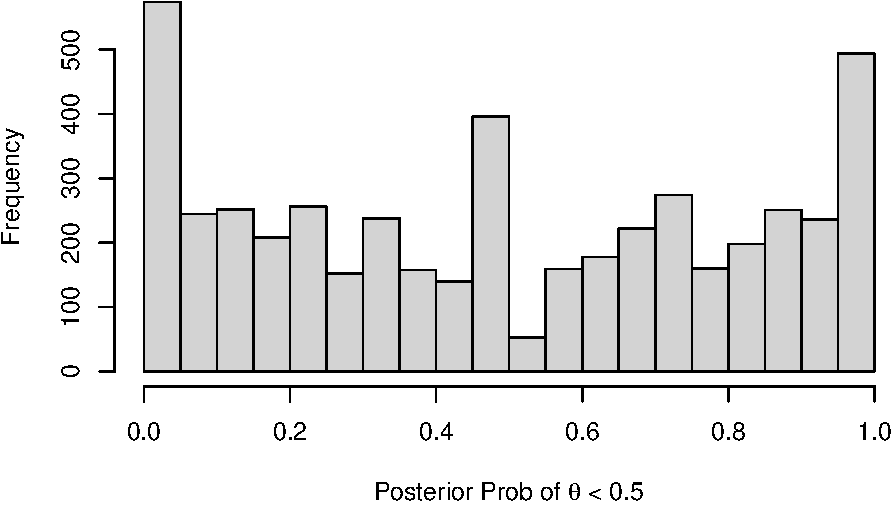
\includegraphics{lab1_files/figure-latex/unnamed-chunk-11-1} \end{center}

Key thing to notice here: the approximation is less good in the long
tail.

\subsection{Distributional summaries}\label{distributional-summaries}

\subsubsection{single-valued summaries: mean, median and
mode}\label{single-valued-summaries-mean-median-and-mode}

There are multiple ways to summarize the central tendency of a
distribution with a single value, including the mean, median, and mode
(the value with the highest probability density). For some distributions
(e.g.~the normal distribution), these values are the same\ldots{}but
that's not always true.

If you're giving a point estimate for a parameter, one of these values
would be what you'd report.

We can calculate those values from the Poisson samples:

\begin{Shaded}
\begin{Highlighting}[]
\CommentTok{# strangely, R doesn't have a built-in function for calculating mode, so we need to code our own:}
\NormalTok{mode <-}\StringTok{ }\ControlFlowTok{function}\NormalTok{(x) \{}
  \KeywordTok{return}\NormalTok{(}\KeywordTok{as.numeric}\NormalTok{(}\KeywordTok{tibble}\NormalTok{(}\DataTypeTok{samples =}\NormalTok{ x) }\OperatorTok
\StringTok{  }\KeywordTok{count}\NormalTok{(samples) }\OperatorTok
\StringTok{  }\KeywordTok{filter}\NormalTok{(n }\OperatorTok{==}\StringTok{ }\KeywordTok{max}\NormalTok{(n)))[}\DecValTok{1}\NormalTok{])}
\NormalTok{\}}

\KeywordTok{mean}\NormalTok{(poisson_samples)}
\end{Highlighting}
\end{Shaded}

\begin{verbatim}
## [1] 4.9746
\end{verbatim}

\begin{Shaded}
\begin{Highlighting}[]
\KeywordTok{median}\NormalTok{(poisson_samples)}
\end{Highlighting}
\end{Shaded}

\begin{verbatim}
## [1] 5
\end{verbatim}

\begin{Shaded}
\begin{Highlighting}[]
\KeywordTok{mode}\NormalTok{(poisson_samples)}
\end{Highlighting}
\end{Shaded}

\begin{verbatim}
## [1] 4
\end{verbatim}

\begin{Shaded}
\begin{Highlighting}[]
\CommentTok{# or use Mode() in package LaplacesDemon}
\NormalTok{LaplacesDemon}\OperatorTok{::}\KeywordTok{Mode}\NormalTok{(poisson_samples)}
\end{Highlighting}
\end{Shaded}

\begin{verbatim}
## [1] 4
\end{verbatim}

Try the same for the gamma samples!

\subsubsection{Intervals}\label{intervals}

We can also use intervals to summarize distributions. In this course we
will place a large focus on \textbf{credible intervals}, which is
constructed based on the (in our case, usually posterior) distribution
of a given parameter. There are two common intervals used to summarize
distributions: percentiles and HDIs (highest density intervals).

\subsubsection{Comparing percentile interval and
HDI}\label{comparing-percentile-interval-and-hdi}

For the Poisson distribution, the 50\% credible intervals has lower
bound the 25\% quantile, and the 75\% quantile as the upper bound:

\begin{Shaded}
\begin{Highlighting}[]
\KeywordTok{summary}\NormalTok{(gamma_samples)}
\end{Highlighting}
\end{Shaded}

\begin{verbatim}
##    Min. 1st Qu.  Median    Mean 3rd Qu.    Max. 
##   0.110   9.591  16.603  19.838  26.492 125.207
\end{verbatim}

\begin{Shaded}
\begin{Highlighting}[]
\KeywordTok{quantile}\NormalTok{(gamma_samples, }\DataTypeTok{probs =} \KeywordTok{c}\NormalTok{(.}\DecValTok{25}\NormalTok{, .}\DecValTok{75}\NormalTok{))}
\end{Highlighting}
\end{Shaded}

\begin{verbatim}
##       25%       75% 
##  9.591237 26.491549
\end{verbatim}

\begin{Shaded}
\begin{Highlighting}[]
\NormalTok{hdi <-}\StringTok{ }\KeywordTok{hdi}\NormalTok{(gamma_samples, }\DataTypeTok{credMass=}\FloatTok{0.5}\NormalTok{)}
\NormalTok{df <-}\StringTok{ }\KeywordTok{data_frame}\NormalTok{(}\DataTypeTok{samples =}\NormalTok{ gamma_samples)}
\NormalTok{p.interval <-}\StringTok{ }\KeywordTok{ggplot}\NormalTok{(df, }\KeywordTok{aes}\NormalTok{(}\DataTypeTok{x =}\NormalTok{ samples)) }\OperatorTok{+}\StringTok{ }\KeywordTok{geom_density}\NormalTok{()}
\NormalTok{p.interval }\OperatorTok{+}\StringTok{ }
\StringTok{  }\KeywordTok{geom_vline}\NormalTok{(}\DataTypeTok{xintercept =} \KeywordTok{quantile}\NormalTok{(gamma_samples, }\DataTypeTok{probs =} \KeywordTok{c}\NormalTok{(.}\DecValTok{25}\NormalTok{, .}\DecValTok{75}\NormalTok{)), }
             \DataTypeTok{color =} \StringTok{"purple"}\NormalTok{, }\DataTypeTok{linetype =} \StringTok{"dashed"}\NormalTok{)}\OperatorTok{+}\StringTok{ }
\StringTok{  }\KeywordTok{geom_vline}\NormalTok{(}\DataTypeTok{xintercept =} \KeywordTok{c}\NormalTok{(hdi[}\DecValTok{1}\NormalTok{], hdi[}\DecValTok{2}\NormalTok{]),  }
             \DataTypeTok{color =} \StringTok{"red"}\NormalTok{, }\DataTypeTok{linetype =} \StringTok{"dashed"}\NormalTok{) }\OperatorTok{+}
\StringTok{  }\KeywordTok{labs}\NormalTok{(}\DataTypeTok{title =} \StringTok{"25%-75% percentile (purple) and 50% HDI (red)"}\NormalTok{)}
\end{Highlighting}
\end{Shaded}

\begin{center}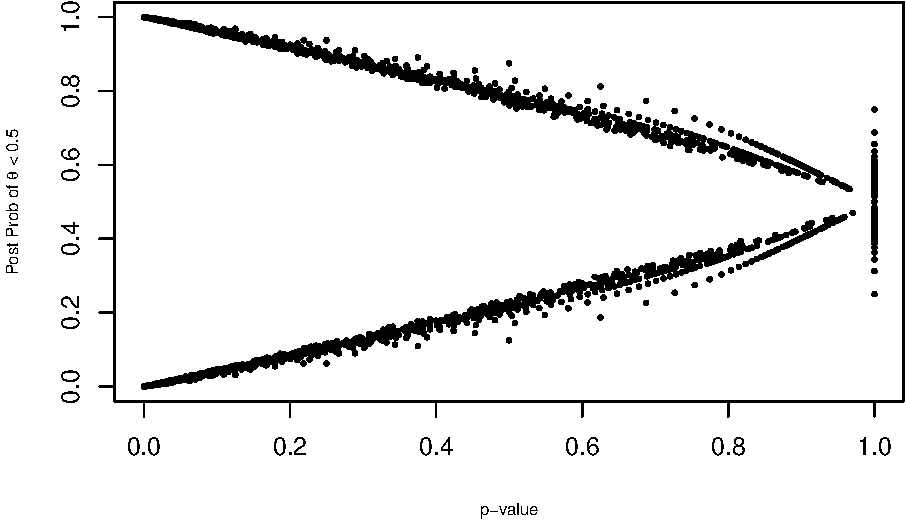
\includegraphics{lab1_files/figure-latex/unnamed-chunk-13-1} \end{center}

\subsubsection{Comparing mean, median and
mode}\label{comparing-mean-median-and-mode}

\begin{Shaded}
\begin{Highlighting}[]
\NormalTok{p.interval }\OperatorTok{+}\StringTok{ }\KeywordTok{geom_vline}\NormalTok{(}\DataTypeTok{xintercept =} \KeywordTok{mean}\NormalTok{(gamma_samples), }\DataTypeTok{color =} \StringTok{"blue"}\NormalTok{) }\OperatorTok{+}\StringTok{ }
\StringTok{  }\KeywordTok{geom_vline}\NormalTok{(}\DataTypeTok{xintercept =} \KeywordTok{median}\NormalTok{(gamma_samples), }\DataTypeTok{color =} \StringTok{"purple"}\NormalTok{) }\OperatorTok{+}\StringTok{ }
\StringTok{  }\KeywordTok{geom_vline}\NormalTok{(}\DataTypeTok{xintercept =}\NormalTok{ LaplacesDemon}\OperatorTok{::}\KeywordTok{Mode}\NormalTok{(gamma_samples), }\DataTypeTok{color =} \StringTok{"red"}\NormalTok{) }\OperatorTok{+}
\StringTok{  }\KeywordTok{labs}\NormalTok{(}\DataTypeTok{title =} \StringTok{"mean (blue), median (purple) and mode (red)"}\NormalTok{)}
\end{Highlighting}
\end{Shaded}

\begin{center}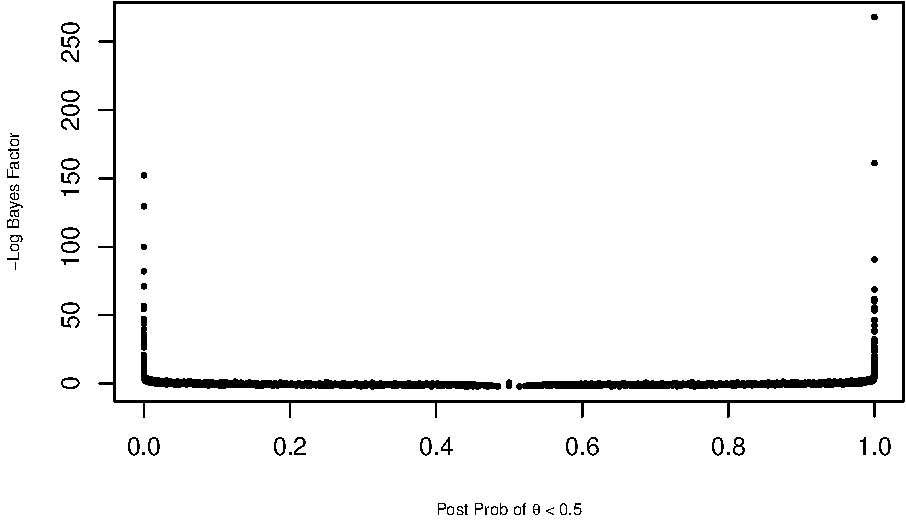
\includegraphics{lab1_files/figure-latex/unnamed-chunk-14-1} \end{center}

What should you use? It depends! The mean is commonly used in Bayesian
statistics, though rstan and bayesplot use the median and percentiles by
default. The mode is less common, but it has a nice correspondence to
the maximum likelihood estimate. In a Bayesian context, this is called
maximum a posteriori estimation.

\subsection{Monte Carlo Simulation}\label{monte-carlo-simulation}

Approximating probability masses and densities through sampling is
called Monte Carlo simulation. For continuous distributions, we're
approximating an integral. You can do this for arbitrary parts of the
distribution:

\[X \sim N(0,1), P(-1 \leq X \leq 1) \approx ?\]

\begin{Shaded}
\begin{Highlighting}[]
\NormalTok{normal_samples <-}\StringTok{ }\KeywordTok{rnorm}\NormalTok{(nsims, }\DataTypeTok{mean =} \DecValTok{0}\NormalTok{, }\DataTypeTok{sd =} \DecValTok{1}\NormalTok{)}

\CommentTok{# how much probability is between -1 and +1 sd in a normal distribution?}
\KeywordTok{sum}\NormalTok{(normal_samples }\OperatorTok{>=}\StringTok{ }\OperatorTok{-}\DecValTok{1} \OperatorTok{&}\StringTok{ }\NormalTok{normal_samples }\OperatorTok{<=}\StringTok{ }\DecValTok{1}\NormalTok{) }\OperatorTok{/}\StringTok{ }\NormalTok{nsims}
\end{Highlighting}
\end{Shaded}

\begin{verbatim}
## [1] 0.679
\end{verbatim}

\begin{Shaded}
\begin{Highlighting}[]
\KeywordTok{pnorm}\NormalTok{(}\DecValTok{1}\NormalTok{) }\OperatorTok{-}\StringTok{ }\KeywordTok{pnorm}\NormalTok{(}\OperatorTok{-}\DecValTok{1}\NormalTok{)}
\end{Highlighting}
\end{Shaded}

\begin{verbatim}
## [1] 0.6826895
\end{verbatim}

Try changing nsims and the lower and upper bounds to see how the
approximation improves.

\section{Poll: Slides or markdown??}\label{poll-slides-or-markdown}

\end{document}
